\thispagestyle{empty}
\onehalfspacing

{\Large
\centerline{\textbf{Univerzita Komenského v Bratislave}}
\centerline{\textbf{Fakulta Matematiky, Fyziky a Informatiky}}
}

\vfil
\vspace{\stretch{1}}
  \begin{center}
    {\LARGE \textbf{Využitie oklúzie v rozšírenej realite}}
    
    \bigskip
    \bigskip

    {\Large Bakalárska práca}\\
  \end{center}
  \vfil

\vspace{\stretch{1}}
\noindent
\begin{tabular}[B]{ll}
Študijný program: & aplikovaná informatika \\
Študijný odbor: & aplikovaná informatika (2511) \\
Školiace pracovisko: & Katedra aplikovanej informatiky \\
Školiteľ:  & RNDr. Zuzana Berger Haladová, PhD. \\
\end{tabular}

\bigskip

\vspace{\stretch{0.1}}
\noindent
\textbf{Bratislava, 2015} \hfill \textbf{Viktor Seč} 	
\pagebreak

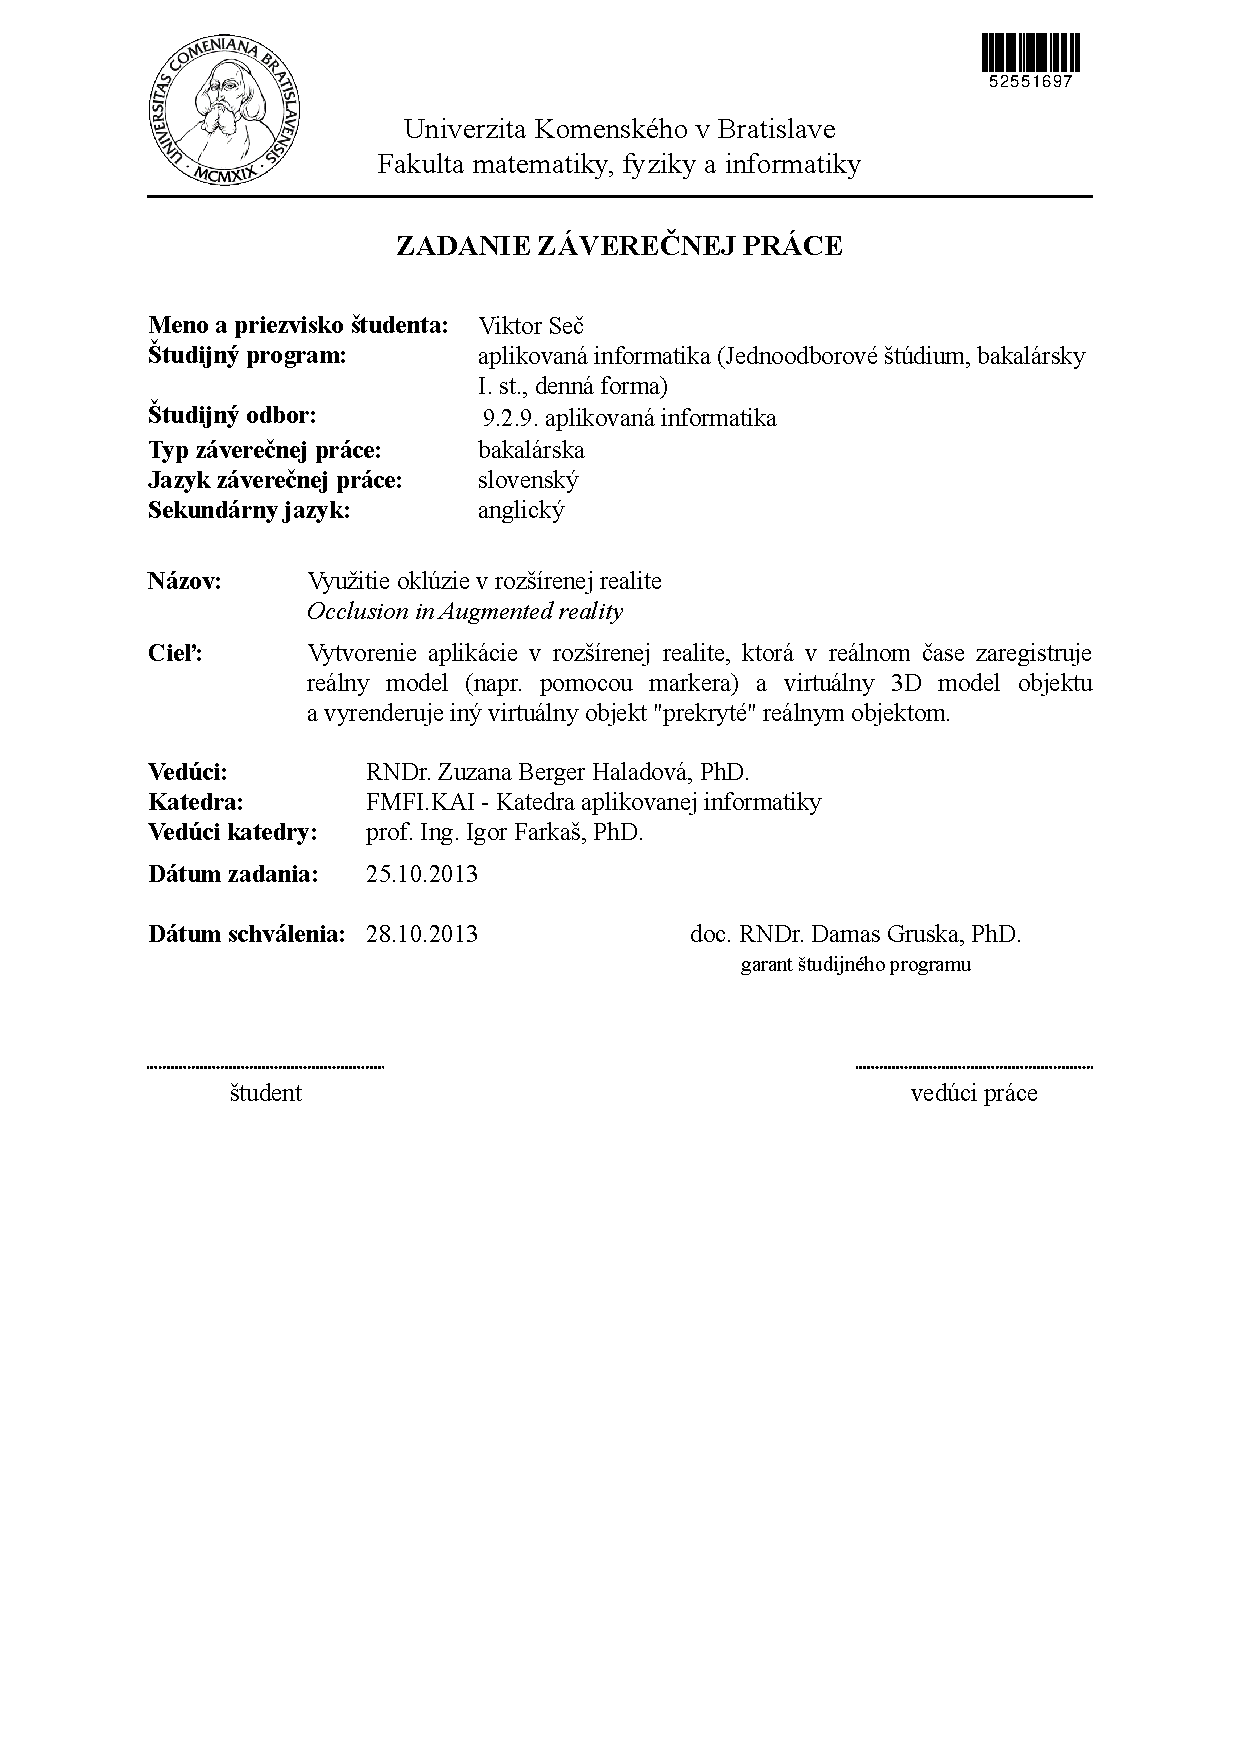
\includepdf[pages={1}]{zadanie.pdf}

%% prehlasenie
\iftrue
	\thispagestyle{empty}
	\vglue0pt

	\vfil

	\noindent\textbf{Čestné prehlásenie}

	\bigskip
	\begin{flushleft}
	Čestne vyhlasujem, že som bakalársku prácu vypracoval samostatne s použitím uvedenej odbornej literatúry.
	\end{flushleft}
	\bigskip

	\noindent Bratislava \today \hfil
	\begin{tabular}[t]{c}
	\hbox to 50mm {\dotfill} \\ \textit{\small Viktor Seč}
	\end{tabular} \qquad \linebreak

	\pagebreak
\fi


